\documentclass{article}
\usepackage[paperwidth=20cm, paperheight=4cm, margin = 0cm, top=0.5cm]{geometry}
\usepackage{amsmath}


\usepackage{pgf}
\usepackage{tikz}


\usetikzlibrary{arrows,automata}

\tikzstyle{source}  = [draw,circle,fill=black,thick,inner sep=0mm,minimum size=2mm]

\renewcommand{\vec}[1]{\boldsymbol{#1}}

\begin{document}
\begin{center}
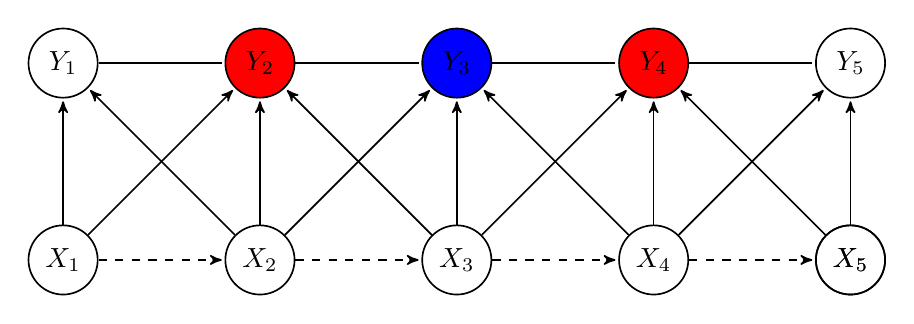
\begin{tikzpicture}[->,>=stealth',shorten >=1pt,auto,node distance=2.5cm,semithick]
                    
\node[state] (X1)               {$X_1$}; 
\node[state] (X2) [right of=X1] {$X_2$};                   
\node[state] (X3) [right of=X2] {$X_3$};                   
\node[state] (X4) [right of=X3] {$X_4$};                   
\node[state] (X5) [right of=X4] {$X_5$};                   
\node[state] (X5) [right of=X4] {$X_5$};                   

\node[state] (Y1) [above of=X1] {$Y_1$}; 
\node[state, fill=red]  (Y2) [above of=X2] {$Y_2$}; 
\node[state, fill=blue] (Y3) [above of=X3] {$Y_3$}; 
\node[state, fill=red]  (Y4) [above of=X4] {$Y_4$}; 
\node[state] (Y5) [above of=X5] {$Y_5$}; 
	
\path
	(X1) edge[dashed] (X2)
	(X2) edge[dashed] (X3)
	(X3) edge[dashed] (X4)
	(X4) edge[dashed] (X5);
	
\path	
	(X1) edge (Y1)
	(X2) edge (Y2)
	(X3) edge (Y3)
	(X4) edge (Y4)
	(X5) edge (Y5);

\path	
	(X1) edge (Y2)
	(X2) edge (Y3)
	(X3) edge (Y4)
	(X4) edge (Y5);

\path	
	(X2) edge (Y1)
	(X3) edge (Y2)
	(X4) edge (Y3)
	(X5) edge (Y4);

	
\path	
	(Y1) edge[-] (Y2)
	(Y2) edge[-] (Y3)	
	(Y3) edge[-] (Y4)	
	(Y4) edge[-] (Y5);	
		
\end{tikzpicture}
\end{center}

\end{document}
